\documentclass[a4paper,11pt]{article}
\usepackage[margin=2cm]{geometry}
\usepackage{graphicx}
\usepackage{color, colortbl}
\usepackage{cite}
\usepackage{url}
\usepackage{float}
\usepackage{arydshln}
\usepackage{pdfpages}
\usepackage{csvsimple}
\usepackage{listings}
\usepackage{algpseudocode}
\usepackage{longtable}
\usepackage{pdflscape}
\usepackage{indentfirst}
\usepackage{mathtools}
\usepackage{amsmath}
\usepackage{amssymb}
\usepackage{tikz}
\usepackage{subcaption}

\definecolor{Green}{rgb}{0.6,1,0.6}
\definecolor{Amber}{rgb}{1,1,0.4}
\definecolor{Red}{rgb}{1,0.6,0.6}

\setlength\parindent{24pt}

\usepackage{fancyhdr}


\title{Some Intuition about Activation Functions in Feed-Forward Neural Networks}


\begin{document}

\maketitle

\abstract
{
Everyone thought it was great to use differentiable, symmetric, non-linear activation functions in feed-forward neural networks, until Alex Krizhevsky \cite{krizhevsky} found that Rectifier Linear Units, despite being not entirely differentiable, nor symmetric, and most of all, piece-wise linear, were computationally cheaper and worth the trade-off with their more sophisticated counterparts. Here are just a few thoughts on the properties of these activation functions, a potential explanation for why using ReLUs speeds up training, and possible ways of applying these insights for better learning strategies.
}

\clearpage

\section{Models of Neurons}

The rectified linear unit is the building block for current state-of-the-art implementations of deep convolutional neural networks. In order to bring out its specific characteristics, we shall first consider two other compatible neuron models: the binary threshold neuron, which is the most intuitive, and the logistic sigmoid neuron, which is the most analytically appealing. \\

\paragraph{Binary Threshold Neuron}
\begin{equation}
y = \begin{cases} 1 & \mbox{if } M <= b + \sum\limits_{i=1}^k x_{i}\cdot w_{i}  \text{ , where } M \text{ is a threshold parameter} \\ 
				  0 & \mbox{otherwise} \end{cases}
\end{equation}

Intuitively, $y$ takes a hard decision, just like biological neurons: either a charge is sent, or it isn't. $y$ can be seen as producing spikes, $x_i$ as the indicator value of some feature, and $w_i$ as a parameter of the function that indicates how important $x_i$ is in determining $y$. Although this model is closer than most most to reality, the function is not differentiable, which makes it impossible to use greedy local optimisation learning algorithms - such as gradient descent - which need to compute derivatives involving the activation functions.

\paragraph{Logistic Sigmoid Neuron} 
\begin{equation}
\label{sigmoid neuron}
y = \frac{1}{1 + e^{-z}} \text{, where } z = b + \sum\limits_{i=1}^k x_{i}\cdot w_{i}
\end{equation}

Like the binary threshold neuron, the output domain of this neuron is bounded by 0 and 1. But this time, the function is fully differentiable. Moreover, it is non-linear, which helps to increase performance \cite{DL-book}.

\begin{figure}[h!]
	\centering
	\begin{subfigure}{.5\textwidth}
  		\centering
		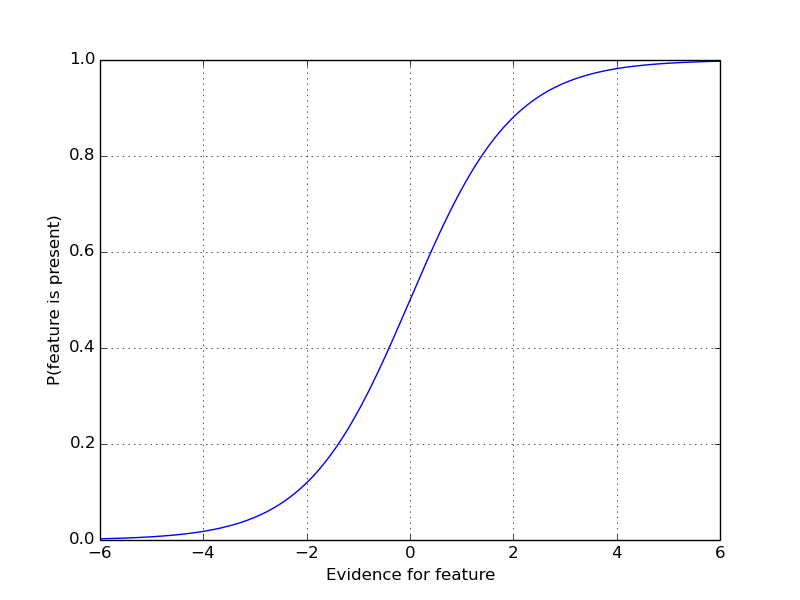
\includegraphics[scale=0.4]{images/logistic.png}
		\caption{Single-Input Logistic Sigmoid Neuron}
	\end{subfigure}%
	\begin{subfigure}{.5\textwidth}
  		\centering
		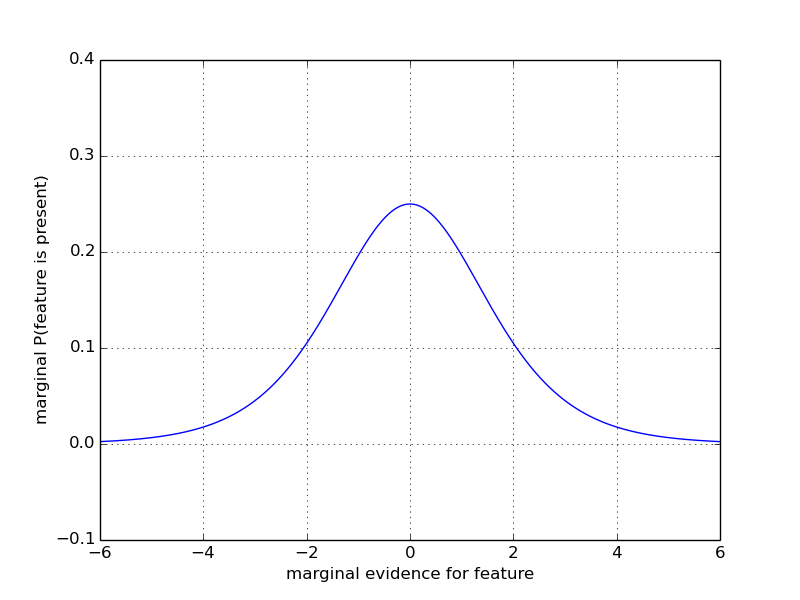
\includegraphics[scale=0.4]{images/logistic-derivative.png}
		\caption{Derivative}
	\end{subfigure}
\end{figure}

\subparagraph{Logistic Unit as a Feature Detector}

To see why the non-linearity of the logistic unit could help to increase performance, the graph plot below lends itself to the following intuition: consider the neuron as a feature detector, where the input x is the amount of evidence for a certain feature, and y is the probability that the feature is present. x is positive if there is evidence in favour of the feature, and negative if against (so $y=0.5$ when $x=0$). y is strictly increasing in x, because every extra amount of evidence for the feature increases the probability of its presence. y is bounded above by 1 and 0, because it is a probability. \\

Interestingly, the slope (i.e.\ the derivative) of y is highest in absolute value around $x=0.5$, and tends towards 0 as x departs from 0.5 in either direction. 

\begin{figure}[h!]
	\centering
\end{figure}

This is like saying: if I'm clueless as to whether the feature is present or not, any evidence in favour of presence or absence will push me easily in that direction; however, the more you want to convince me of it, the higher the required evidence gets. One can imagine a number of situations involving hypothesis evaluation where this kind of 'attitude' is adopted (a jeweller will put disproportionately more effort into checking that a stone is 64 carat than checking that it is 32 carat, it takes disproportionately more effort to push one's expected exam grade from 80 to 84 than from 40 to 44, it take disproportionately more persuasion for an investor to raise the proportion of personal funds invested in a single project from 96\% to 100\% than from 0\% to 4\%, etc). \\

It may be interesting to consider how choosing a logistic activation function impacts back-propagation of the gradient during training of a feed-forward neural network. Before doing so however, the rectified linear neuron will be introduced, followed with how the gradient back-propagates through a feed-forward neural network during training. \\
                
\paragraph{Rectified Linear Neuron}
\begin{equation}
\label{relu}
y = \max\{0, b + \sum\limits_{i=1}^k x_{i}\cdot w_{i}\}
\end{equation}

As can be seen in the graph plot below, the rectified linear neuron is neither fully differentiable (not at $0$), nor bounded above. Moreover, its derivative can only take two values, $0$ or $1$. Although this may come as a strong downgrade in sophistication compared to the logistic sigmoid neuron, it is so much more efficient to compute (both its value and its partial derivatives) that it enables much larger network implementations\cite{krizhevsky}. Until now, this has more than offset the per-neuron information loss - and saturation risks - of the rectifier versus the sigmoid unit \cite{rectifier}. Most importantly, using ReLUs rather than logistic units considerably speeds up training \cite{krizhevsky}. Mathematical intuition for this will be proposed later down.

\begin{figure}[h!]
	\centering
	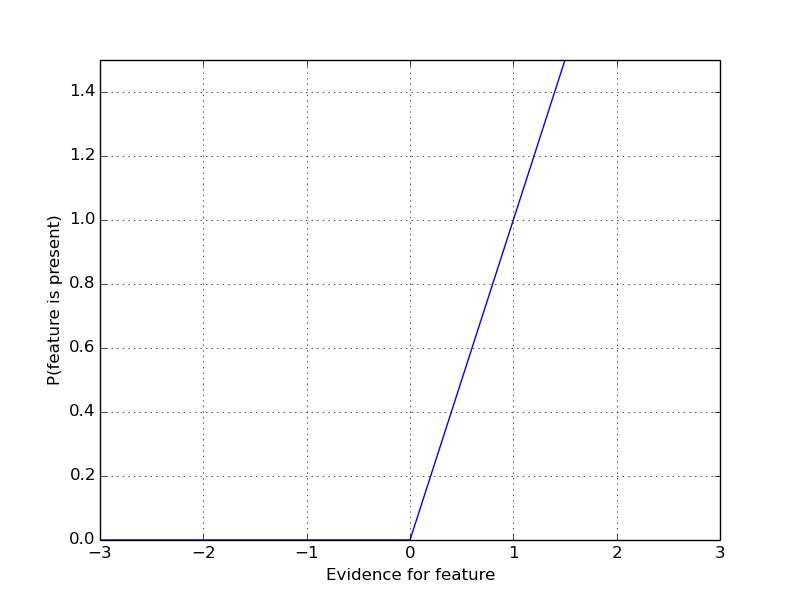
\includegraphics[scale=0.5]{images/ReLU.png}
	\caption{Single-Input Rectified Linear Neuron}
\end{figure}

It may seem almost staggering that an unbounded activation function can be used to train a network without getting exploding output or saturated regions. (Need to see whether research has been done on this, but I managed to ask Yann LeCun in person, and he was unsure of why).


\section{Training: Backpropagation}

The parameters (a.k.a\ weights) of feed-forward neural networks in the context of supervised learning are trained with backpropagation, which makes use of gradient descent: a weight $w$ is adjusted by $\tau \cdot \frac{\partial{E}}{\partial{w}}$, which is a multiple of the error, and this multiple is determined by the weights and neurons that lie in the paths from the weight to a neuron of the output layer. The choice of activation function will modify the formula for a weight update, so the comparison between the logistic unit and the ReLU extends to training.

\subsubsection{How the Gradient Propagates}

It may be of interest to know how the gradient propagates through a network - especially since a single vector of information - the error - is supposed to adjust up to millions of parameters, which could be considered as a bit of a stretch.\\

With the following notation:
\begin{itemize}
\renewcommand\labelitemi{--}
\item $y_{j}$, the output of unit (a.k.a\ neuron) $j$, but also used to refer to the unit $j$ itself
\item $w_{ij}$, the weight of the edge connecting lower-layer neuron $y_{i}$ to upper-layer neuron $y_{j}$
\item $z_{j} := b+ \langle x,w \rangle = b + \sum\limits_{i=1}^k x_{i}\cdot w_{ij}$, the input vector for $y_{j}$
\item $\psi$, the activation function used -- therefore $y_{j} = \psi(z_{j})$ \\
\end{itemize}

The rules for propagating the gradient backwards through a network are:
\begin{itemize}
\renewcommand\labelitemi{--}
\item to \textbf{initialise}: $grad \leftarrow \mathcal{C}'(y_{L})$, where $y_{L}$ is the output unit
\item to \textbf{propagate through a unit} $y_{j}$: $grad \leftarrow grad \cdot \psi'(z_{j})$
\item to \textbf{propagate through an edge} $w_{ij}$: $grad \leftarrow grad \cdot w_{ij}$
\item to \textbf{stop at an edge} $w_{ij}$: $grad \leftarrow grad \cdot y_{i}$ \\
\end{itemize}


\begin{figure}[h!]
	\centering
	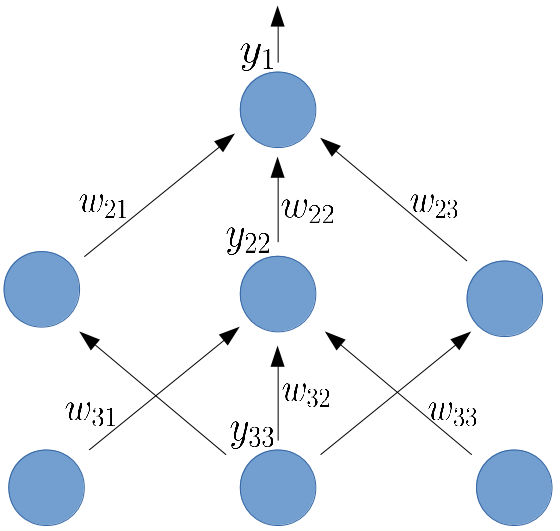
\includegraphics[scale=0.28]{images/gradient_propagates.png}
	\caption{(CHANGE NOTATION to reflect one above with $\textbf{y}_L$ for top layer) Feed-Forward Neural Network with one Hidden Layer}
\end{figure}

So for example, given the figure above:
\begin{itemize}
\renewcommand\labelitemi{--}
\item for $\frac{\partial{E}}{\partial{w_{57}}}$: initialise, propagate through $y_{7}$, then stop at $w_{57}$:
 $ \mathcal{C}'(y_{7}) \cdot \psi'(z_7) \cdot y_5$ 
\item for $\frac{\partial{E}}{\partial{w_{25}}}$: initialise, propagate through $y_{7}$, $w_{57}$, $y_{5}$ then stop at $w_{25}$:
 $\mathcal{C}'(y_{7}) \cdot \psi'(z_7) \cdot w_{57} \cdot \psi'(z_5) \cdot y_2$ \\
\end{itemize}

Notice that if $y_7$ is 

\subsubsection{ReLUs Train Faster}

Networks consisting of ReLUs have empirically trained faster than those consisting of sigmoid units. This may be because if a sigmoid unit is in its saturated environment, its weights are harder 

\begin{figure}[h!]
	\centering
	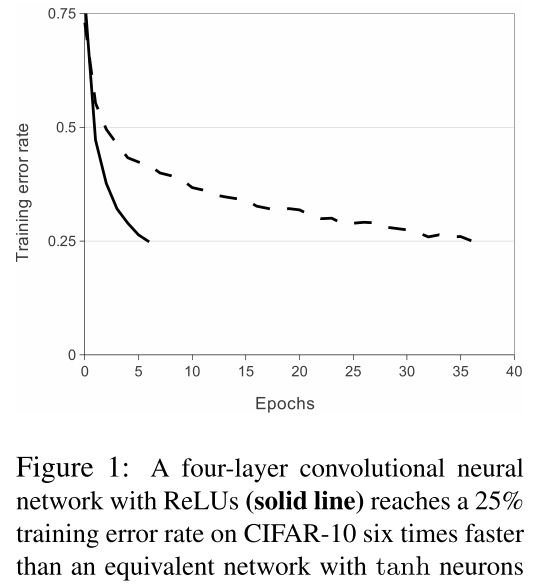
\includegraphics[scale=0.3]{images/ReLU_train_fast.png}
	\caption{Training AlexNet (Krizhevsky et al 2012)}
\end{figure}

\begin{thebibliography}{1}
% Example: \bibitem{One}
% a better way of doing it: a .bib file or something. bit.ly/1kqg2Qe
\bibitem{decaf}
 Donahue, Jeff; Jia, Yangqing; Vinyals, Oriol; Hoffman, Judy; Zhang, Ning; Tzeng, Eric; Darrell, Trevor;
  \emph{DeCAF: A Deep Convolutional Activation Feature for Generic Visual Recognition}\\
  arXiv preprint arXiv:1310.1531, 2013

\bibitem{MIML}
 Zhou, Zhi-Hua; Zhang, Min-Ling;
  \emph{Multi-Instance Multi-Label Learning with Application to Scene Classification}\\
  Advances in Neural Information Processing Systems 19, 
  Proceedings of the Twentieth Annual Conference on Neural Information Processing Systems, 
  Vancouver, British Columbia, Canada, 
  December 4-7, 2006

\bibitem{f-measure}
 Pastor-Pellicer, Joan; Zamora-Martinez, Francisco; Espana-Boquera, Salvador; Castro-Bleda, Maria Jose;
  \emph{F-Measure as the Error Function to Train Neural Networks}\\

\bibitem{control-point}
 Fusion Group - ControlPoint LLP,
 \emph{Company Description}\\
 URL: \url{http://www.fusionprovida.com/companies/control-point}, last accessed 5th June 2014. 
  
\bibitem{univ-approx}
 Barron, Andrew R.,
 \emph{Universal Approximation Bounds for Superpositions of a Sigmoidal Function}\\
 IEEE Transactions on Information Theory, 
 Vol. 39, No. 3
 May 1993

\bibitem{DL-book}
 Bengio, Yoshua;
 \emph{Learning Deep Architectures for AI}\\
 Foundations and Trends in Machine Learning, 
 Vol. 2, No. 1 (2009) 1-127
 2009

\bibitem{Russel & Norvig}
 Russell, Stuart J; Norvig, Peter;
 \emph{Artificial Intelligence: A Modern Approach}\\
 2003

\bibitem{krizhevsky}
 Krizhevsky, Alex; Sutskever, Ilya; Hinton, Geoffrey E.;
 \emph{ImageNet Classification with Deep Convolutional Neural Networks}\\
 2012

\bibitem{rectifier}
 Glorot, Xavier; Bordes, Antoine; Bengio, Yoshua;
 \emph{Deep Sparse Rectifier Neural Networks}\\
 2013

\bibitem{MLP-univ-approx}
 Hornik, Kur; Stinchcombe, Maxwell; White, Halber;
 \emph{Multilayer Feed-Forward Networks are Universal Approximators}\\
 1989

\bibitem{office}
 Saenko, K., Kulis, B., Fritz, M., and Darrell, T.;
 \emph{Adapting visual category models to new domains}\\
 ECCV, 2010

\bibitem{surf}
 Bay, H., Tuytelaars, T., and Gool, L. Van;
 \emph{SURF: Speeded up robust features}\\
 ECCV, 2006

\bibitem{transfer-learning}
 Sermanet, Pierre; Eigen, David; Zhang, Xiang; Mathieu, Michael; Fergus, Rob; LeCun, Yann;
 \emph{OverFeat: Integrated Recognition, Localization and Detection using Convolutional Networks}\\
 arXiv:1312.6229
  
\bibitem{f-measure}
 Joan Pastor-Pellicer, Francisco Zamora-Martínez, Salvador España-Boquera, María José Castro-Bleda;
 \emph{F-Measure as the Error Function to Train Neural Networks}\\
 Advances in Computational Intelligence
 Volume 7902, 2013, pp 376-384
 
\bibitem{cuda-convnet}  
 URL: \url{https://code.google.com/p/cuda-convnet/}, last accessed 6th June 2014.

\end{thebibliography}

\end{document}
